\chapter{Kernel CN:\ Static semantics}%

\margintoc{}%
%
I have covered a large amount of background to the type system so far:
\intro{Core}, liquid types, bidirectional type systems, linear types, precise
separation logic assertions, monadic syntax for the latter and its relation to
kernel syntax for types, let-normalisation and explicit resource terms in
\kl{ResCore}. I use all of these ingredients in defining the type system for
\kl{kernel CN} that I will explain in this chapter. Some of the sections will
based on my contributions to~\sidetextcite[4.5cm]{pulte2023cn}%

The \kl{Kernel CN} type system is ordinary \kl{CN}, defined over \kl{ResCore}
instead of \kl{Core}, without any type or resource inference. In particular, It
requires that that all universal quantifiers are explicitly instantiated, that
all existential quantifiers have explicit witnesses, and all resource
operations are embedded into the program itself as linearly typed proof terms.
It does not require proof terms for the logical properties, since by
construction all of the entailments fall into the decidable SMT fragment; many
rules rely on this. The lack of inference make it a simpler language for which
to prove type soundness, whilst still demonstrating all the key ingredients
mentioned above. Since it handles the majority of C, the entire system is very
large, and so I will only discuss the main features.

There are some additional minor differences between the implementation and the
formalisation. As I mentioned \nameref{sec:desugaring}, the formalisation has a
richer grammar of resources: this makes defining predicates to represent tagged
unions more succinct, and allows for opening predicates in more cases. The
formalisation assumes that iterated resources output arguments have type array
of records, whereas the implementation uses records of arrays.\sidenote{This
purely a notational convenience so I could avoid inventing syntax for indexing
over an arbitrary record of arrays.}

Along with the type system, I briefly discuss a formalisation of two different
elaboration algorithms: one for inferring instantiations of logical quantifiers,
one for inferring indices for \kl{iterated} predicates. Because of a change
to the inference scheme used by \kl{CN}, the latter algorithm is no longer
used.\sidenote{\href{https://github.com/rems-project/cerberus/commit/7c2c0a364a4373e4eb109f32d01cc9584f51e81f}{Commit
7c2c0a36.}}\label{sn:new-inf-statics}

\section{Contexts}

The contexts for the static semantics consist of four parts: (1) $\mathcal{C}$
containing the computational variables from the Core program; (2) $\mathcal{L}$
containing purely logical variables mentioned in specifications; (3) $\Phi$,
the constraint context, containing a list of (non-quantified) SMT constraints;
and (4) $\mathcal{R}$ a \emph{linear} context containing the resources
available at that point during type-checking. I assume a constraint context of
only non-quantified constraints because users are required to manually
instantiate quantified constraints to use them.

\section{Pure values and expressions}

\kl{ResCore} programs have both computational and logical (ghost) terms.
Every such term, computational or ghost, has a \kl{base type} $\beta$,
which are things like unit, booleans, (mathematical) integers,\sidenote{After the formalisation was completed,
\kl{CN} switched from using mathematical unbounded integers to bit vectors
(\href{https://github.com/rems-project/cerberus/commit/8fdd4198750446de3b44d00f9e8f185db9610fab}{around
commit 8fdd41987}) to better support common bit-twiddling idioms, used heavily
in the buddy allocator in pKVM, without resorting to lots of lemmas about
uninterpreted functions.} locations, and records and user-defined algebraic datatypes of
other base types. Each C type $\tau$ is mapped to a corresponding base type $\beta_\tau$
\textemdash{} for example, $\beta_{\mathtt{int*}} = \mathsf{loc}$.

Logical terms are variously referred to as ${term}$, ${iguard}$ (for boolean
index guards of iterated predicates), ${ptr}$ (for pointers), ${init}$ (for
initialisation status), ${value}$ (for pointees), ${iarg}$ (for input mode
arguments to predicates),  ${oarg}$ (for output arguments for type record or
array of records), and later, ${alloc}$ (for constraints about the allocation
history).

As seen in \cref{fig:typing-pval-pexpr}, the rules for pure
values\sidenote{Because \kl{Core} factors out the memory object model, it also
factors out the precise representation of memory objects such as integers,
pointers, arrays and structs, so I have followed a similar factorising in
the structure of the typing judgements, and left the representation of these
values abstract.} are very simple pure value synthesis judgements of the form
$\mathcal{C} \vdash \mathit{pval} \Rightarrow \colorbox{red!8}{\beta}$;
given computational context and a pure value, synthesise a base type.

Building on the rules for pure values, the pure expression synthesis judgements
are not that much more complicated either: $\mathcal{C}; \mathcal{L}; \Phi
\vdash \mathit{pexpr} \Rightarrow \outpol{pure\_ret}$. Given a computational
context, a logical context, a constraint context and a pure expression,
synthesise a \emph{pure} return type (a return type without any resources or
logical variables). The use of return types starts to introduce a few more of
the refinement type features gestured at earlier. The type $\Sigma y {:}
\beta.\ \phi(y) \wedge{} I$ is simply the usual refinement type $\{ \, y \in
\beta \mid\phi(y) \, \}$, translated over to the grammar of types in \kl{Kernel
CN}. Recall that $\Sigma$ is used to bind a computational value in a
\emph{return} type, so these types are simply expressing, symbolically, in
constraints, that these expressions will evaluate to a value. Pure values are
simply lifted into the grammar of SMT constraints with an equality constraint;
pure expressions are lifted similarly but with their equivalent symbolic
computation.

\begin{figure*}[tp]
    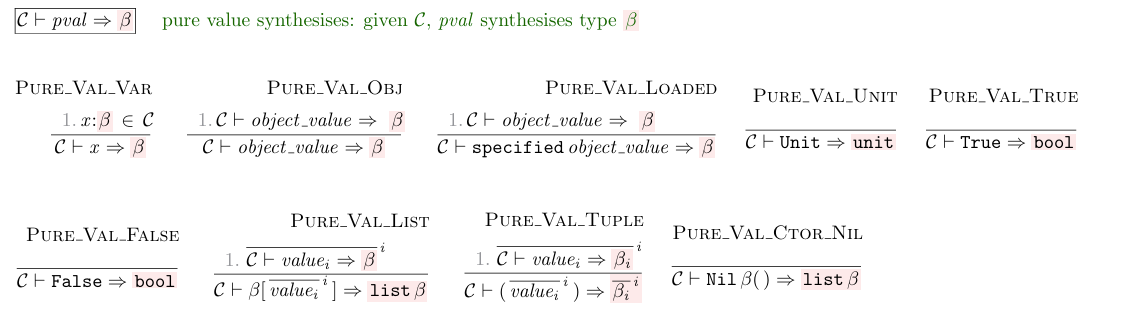
\includegraphics{figures/kernel-pval-typing}
    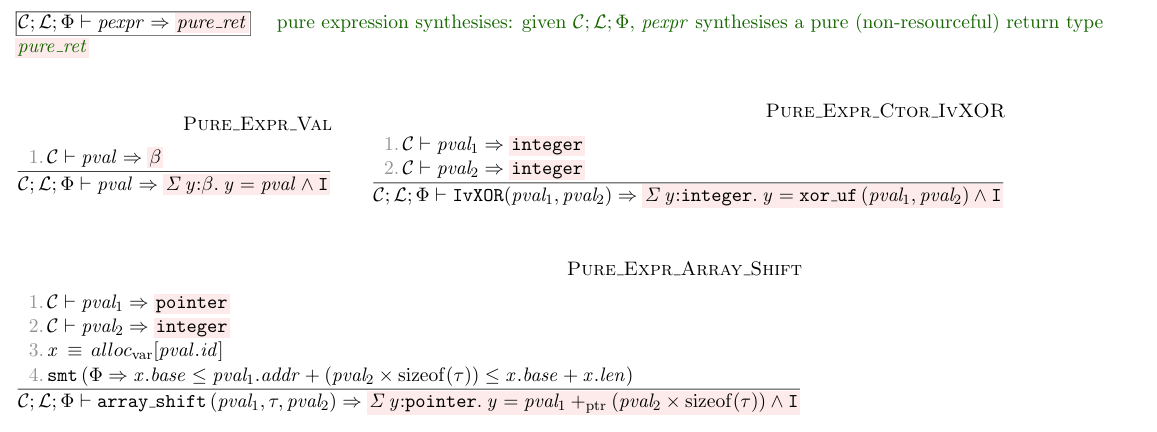
\includegraphics{figures/kernel-pexpr-typing}
    \caption{Selection of \kl{Kernel CN} typing rules for pure values and
        expressions.}\label{fig:typing-pval-pexpr}
\end{figure*}

\section{Top-level pure value values and expressions}

Whilst the rules for typing \emph{top-level} pure values and pure expressions
share the same context as typing pure values and expressions, they differ in
that they are \emph{checking} judgements instead of synthesising ones, of the
form $\mathcal{C}; \mathcal{L}; \Phi \vdash \mathit{tpexpr} \Leftarrow
\mathit{pure\_ret}$ (and similarly for $\mathit{tpexpr}$). Given the
computational, logical and constraint contexts, check the top-level value (or
expression) has satisfies this type.

Here we start to see the let-normalisation (\cref{sec:rescore}) and the
bidirectional (\cref{sec:bidir-subtyping}) approaches pay off. A top-level pure
value (i.e.\ the result of evaluating a pure expression) is checked against a
pure return type by checking if the constraint attached to it is true given the
context by calling the SMT solver, which is another reason why the constraints
being decidable is important and helpful. Similarly, the constructs we would
like to avoid (\coreinline{undef()} and \coreinline{error()}) check against % chktex 36
\emph{any} type, so long as the constraint context is inconsistent (can prove
$\mathsf{false}$). Top-level if-expressions synthesise a type for their condition,
but then check the branches, with an extra constraint on the true or false
value of the condition. Similarly, top-level let-expressions synthesise a type
for the bound expressions, and a constraint on the \emph{shape} bound value to
the context, and then check the body of the let.

The constraint on the shape of the bound value is produced by a judgement which
given a computational pattern (one inherited from Core) and a base type, it
produces a computational context and a term corresponding to the \emph{shape}
of the value according to the pattern match. For the sake of simplicity, I
assume all patterns are complete.

\begin{figure*}[tp]
    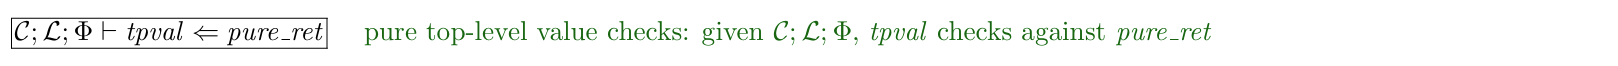
\includegraphics{figures/kernel-tpval-typing}
    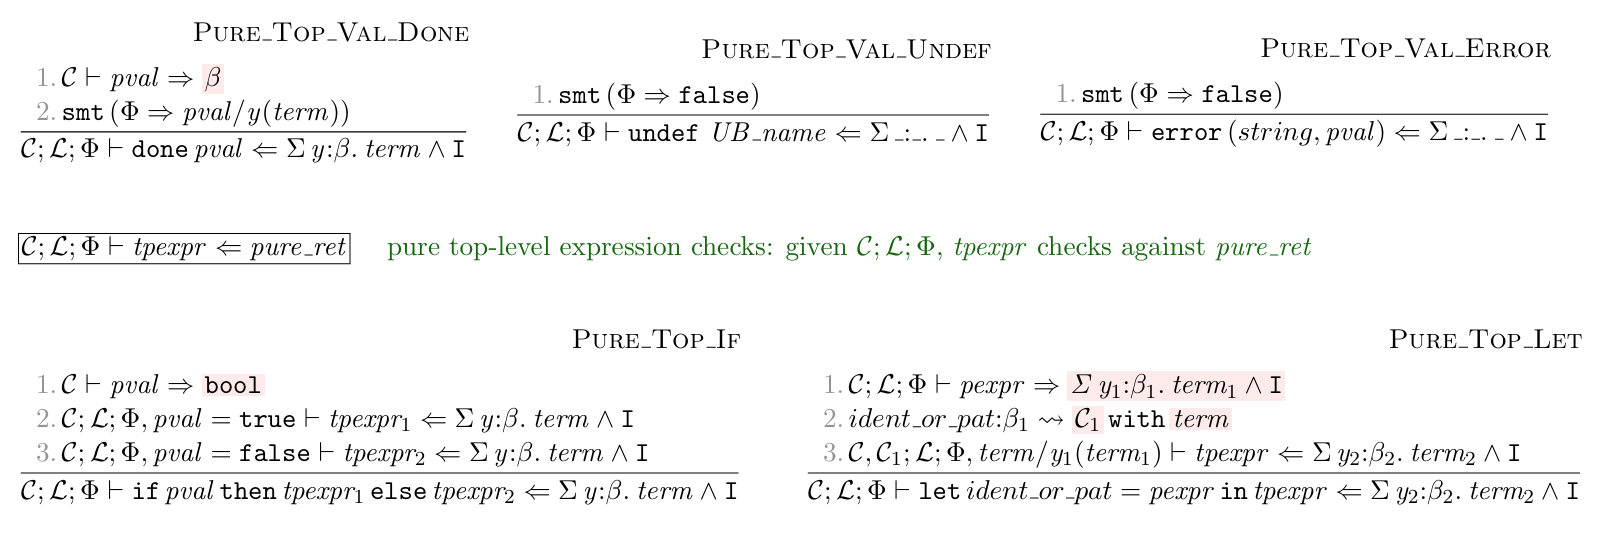
\includegraphics{figures/kernel-tpexpr-typing}
    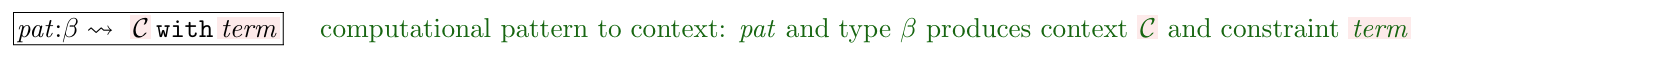
\includegraphics{figures/kernel-pat-comp-typing-1}
    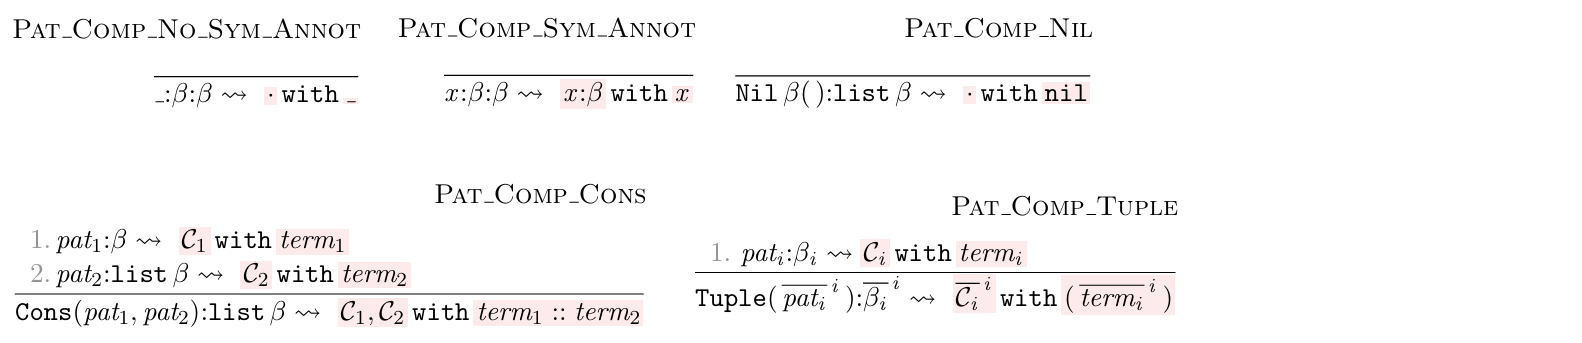
\includegraphics{figures/kernel-pat-comp-typing-2}
    \caption{Selection of \kl{Kernel CN} typing rules for top-level pure values and
        expressions, including the translation of computational patterns into a
        computational context used in the \coreinline{let} rule.}\label{fig:typing-tpval-tpexpr}
\end{figure*}

\section{Resource terms}\label{sec:typing-res-terms}

\begin{figure*}[tp]
    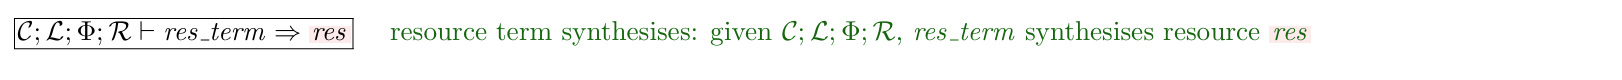
\includegraphics{figures/kernel-res-term-synth-1}
    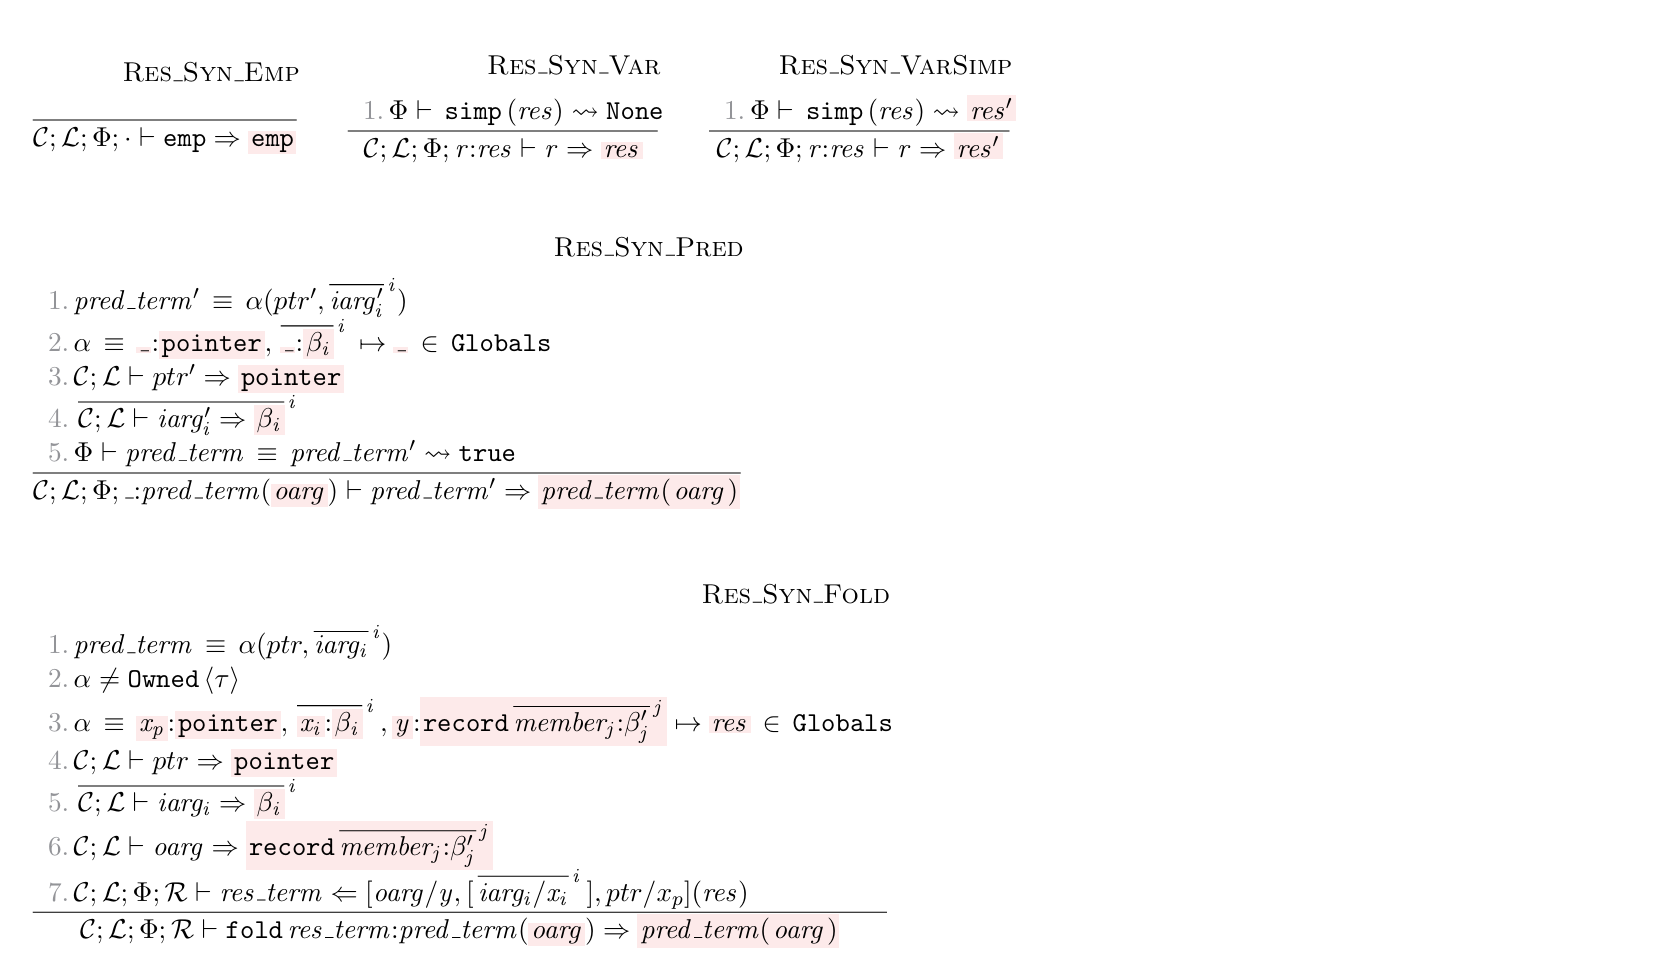
\includegraphics{figures/kernel-res-term-synth-2}
    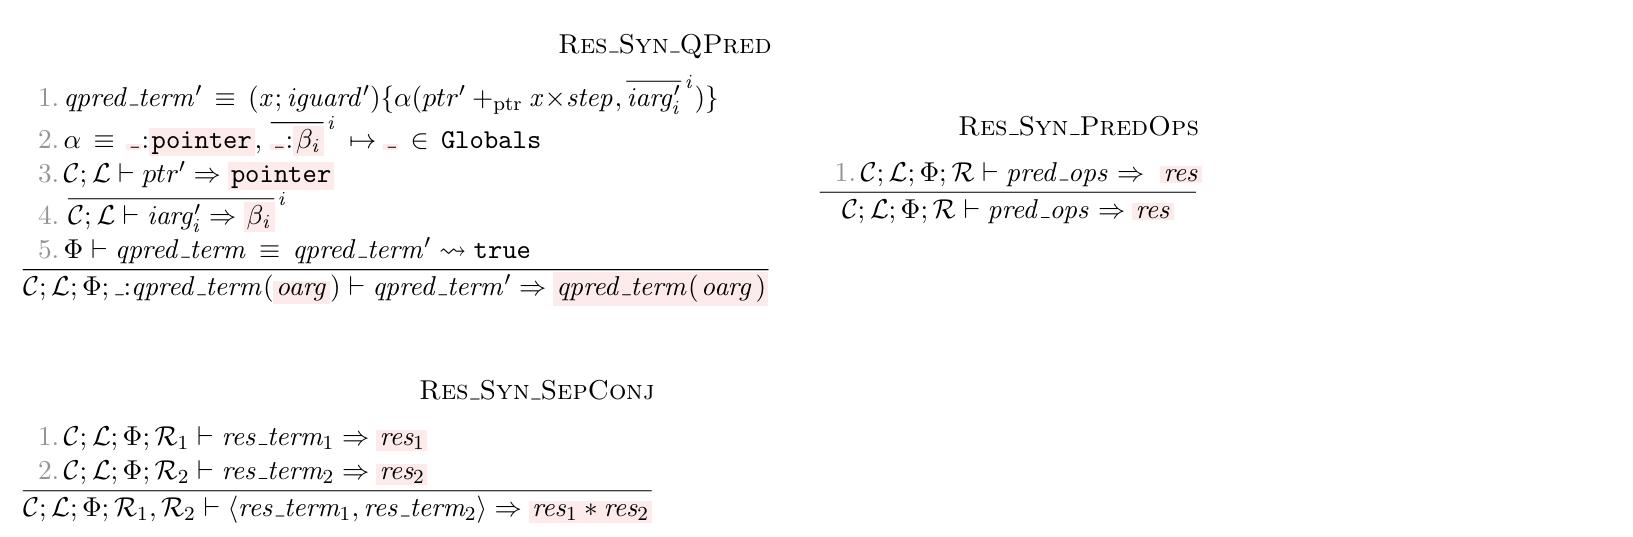
\includegraphics{figures/kernel-res-term-synth-3}
    \caption{Selection of \kl{Kernel CN} synthesising typing rules for resource
        terms.}\label{fig:typing-res-term-synth}
\end{figure*}

Typing resource terms requires the addition of an extra \emph{linear} context
$\mathcal{R}$ of resources. I will start with the synthesising judgements first,
and move on to checking judgements after.

\subsection{Synthesis for resource terms}

As visible in \cref{fig:typing-res-term-synth}, unsurprisingly, $\mathsf{emp}$
requires an empty context, and a variable use requires a singleton context.
Using variables also \emph{simplifies} them; simplification here just means
stripping as many top-level \coreinline{if}s off when their conditions are
provable to be true or provable to be false. Predicate (iterated and otherwise)
terms synthesise their types by checking the arguments (input and output) are
of the correct type. Note that (a) because of linearity, the context is a
singleton and (b) the lookup into the context is by predicate name $\alpha$ and
its input arguments, not by variable and (c) the output argument is synthesised
from the context. For ownership predicates, the input is the location, but the
output will be the initialisation status and the value stored at that location:
the program terms are not required to know what is in the heap.

Only user-defined predicates can be folded, so $\mathsf{Owned}\langle\_\rangle$
is excluded.\sidenote{Needs to be updated for $\mathsf{Alloc}$ too.} A term to
be folded is simply the (partially-evaluated) body of some predicate, so it
does not have the information required to know which predicate it could belong
to, especially because resources can and are moved between predicate. Hence,
morally, $\mathsf{fold}$ should be checked, not synthesised. However, in a
prior version of \kl{CN}, users were required to manually fold and unfold
predicates, and the placement of that annotation was done in an
indeterminately-sequenced expression, which also includes things like memory
actions. Memory actions are not well suited to be checked and are best
synthesised, and so this forced the fold/unfold annotations, and the resource
terms it contained, to also be synthesising.\sidenote{Of course, despite all
this, because the resource assertions are all assumed to be precise, we
could infer the output argument, but {Kernel CN} is meant to assume no
inference of instantiations to logical quantifiers, i.e.\ output arguments of
resources.} Hence, $\mathsf{fold}$ terms are annotated with the predicate which
they are meant to be folded into, so that the $\mathit{res\_term}$ it carries
can be \emph{checked} against the \emph{definition} (`body') of that predicate,
with the input and output arguments substituted in (after the arguments
are checked to be of the correct type).

\subsection{Synthesis for predicate operations}

Predicate operations are also synthesising and have their own judgement. And
because these operations can combine more than one kind of resource, they need
to synthesise separating conjunctions, so the rule for them is also
synthesising.

For space, I only present the rules for turning ownership of fixed size array
into an iterated separating conjunction and back (\cref{fig:typing-predops}).

The first rule says that if $\mathit{res\_term}$ synthesises ownership of a
fixed size array, then the iteration of that synthesises an iterated separating
conjunction for ownership over the indices of that array ($0$ to
$n-1$).\sidenote{The notational hacks in this rule are a bit too cute and
difficult to explain, should probably change them.} The second rule does the
inverse, but includes some additional checks to prevent two adjacent locations
of the same type but belonging to different allocations, being indexable from
a single base pointer.

\begin{figure*}[tp]
    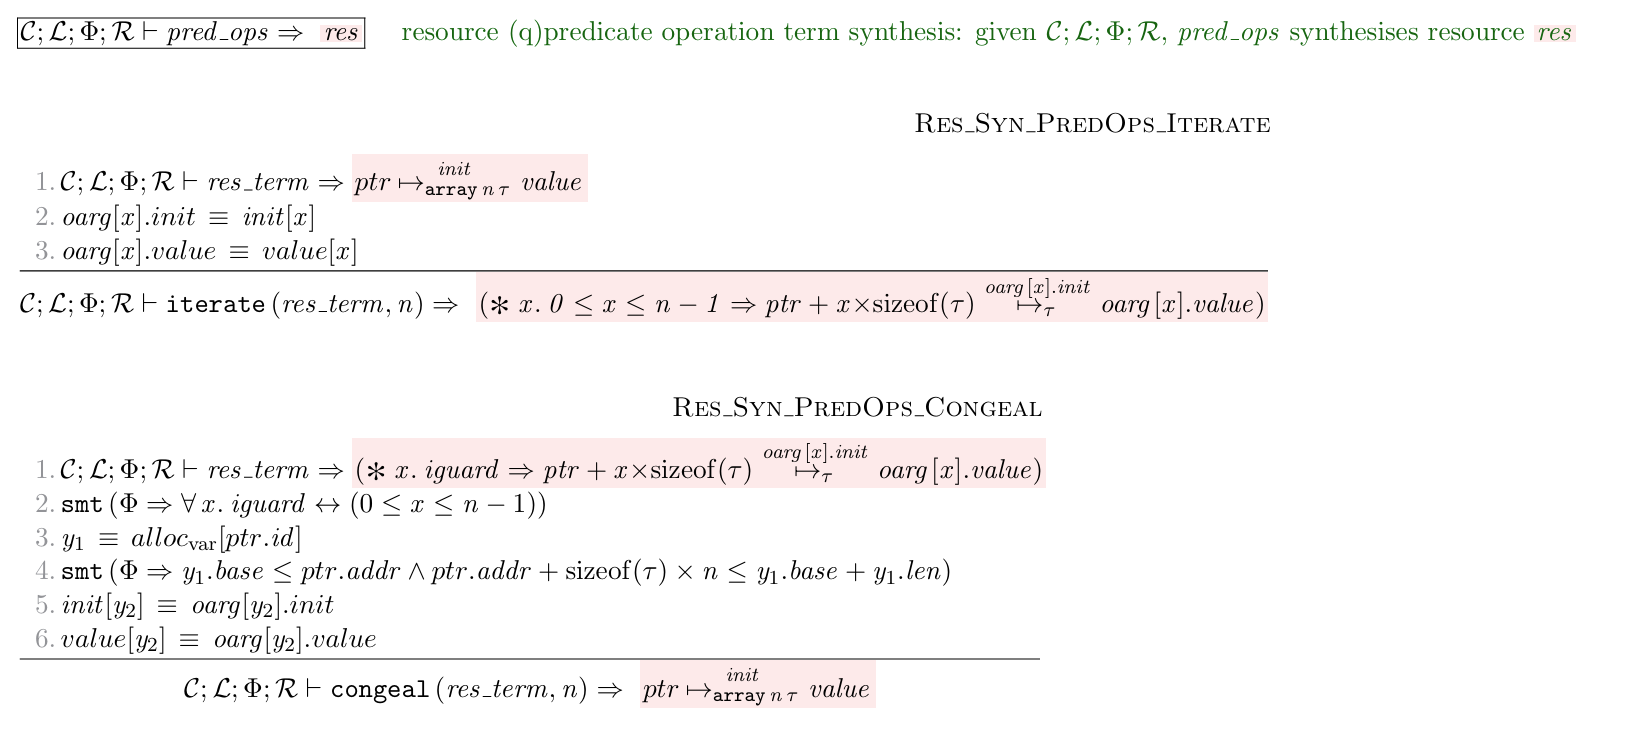
\includegraphics{figures/kernel-predops-typing}
    \caption{Selection of \kl{Kernel CN} synthesising typing rules for
        predicate operations.}\label{fig:typing-predops}
\end{figure*}

\subsection{Checking for resource terms}

Lastly for the resource terms, we come to the checking rules. Resource terms
which represent constraints do not carry the constraint in them, and so need a
checking rule to learn them and prove them with a call to the SMT solver.
Similarly, because it is impossible to infer existential types in the general
case,\sidenote{Consider a heap $1 \mapsto 1$, and consider that all of $\exists
x.\ 1 \mapsto 1$, $\exists x.\ x \mapsto 1$, $\exists x.\ 1 \mapsto x$
(imprecise), $\exists x.\ x \mapsto x$ are valid inferences for it.} this too
is checking, and is straightforward since the instantiation is part of the
term, so it can be substituted into the type, which in turn can check the
$\mathit{res\_term}$ it carries.

As I mentioned earlier (\cref{subsec:res-terms}), \emph{any} resource term can
introduce an ordered-disjunction, and so any resource term can be checked by
it. Furthermore, at most \emph{one} of the branches may be checked, and which
one depends on whether the condition or its negation can be proven. In the
situation that neither is possible, I call the condition (and the resource)
\intro{under-determined} (with respect to a constraint context). In this case,
the system may attempt to synthesise a type for the term and check that the
synthesised type is equal to the ordered disjunction. Only variables can
synthesise an ordered-disjunction type, that too only if the condition is
under-determined (otherwise simplification will reduce it to either branch).
Separating conjunctions are also checked to allow for the case where an
existential or an ordered-disjunction are in the sub-components.

\begin{figure*}[tp]
    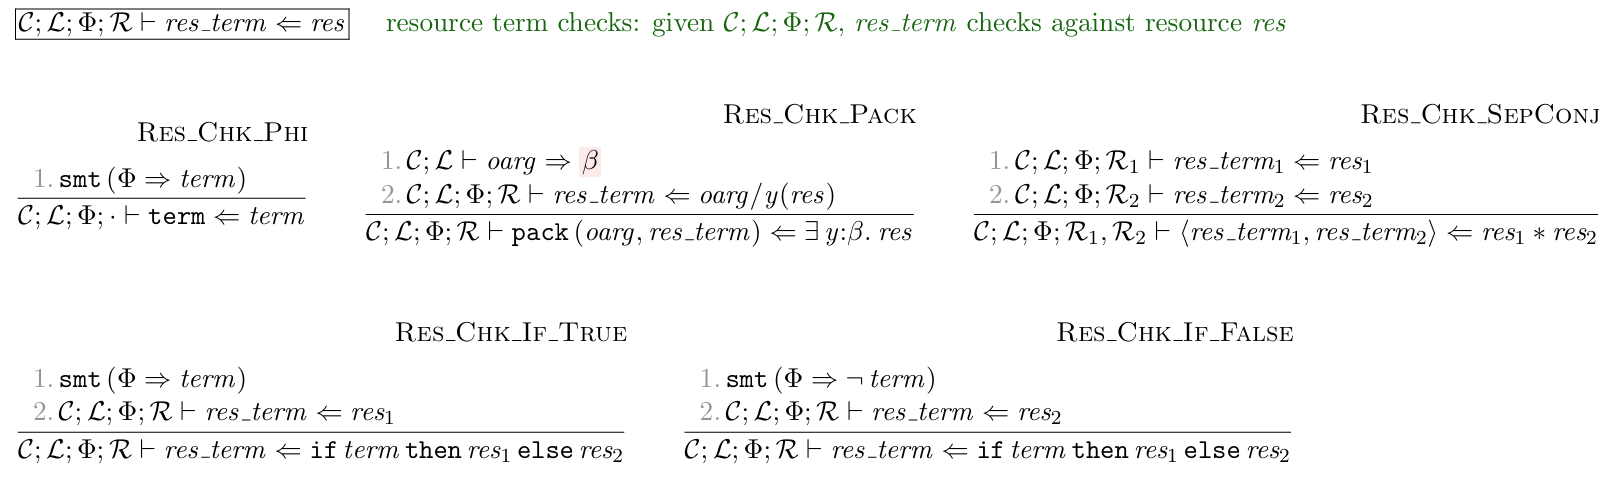
\includegraphics{figures/kernel-res-term-check}
    \caption{Selection of \kl{Kernel CN} checking typing rules for
        resource terms.}\label{fig:typing-res-term-check}
\end{figure*}

At any point, if the term cannot be checked by any other rule, the system can
switch to synthesising a type and then comparing whether the two types are
structurally equal, modulo SMT provability (\cref{fig:typing-res-term-check}).

\begin{marginfigure}
    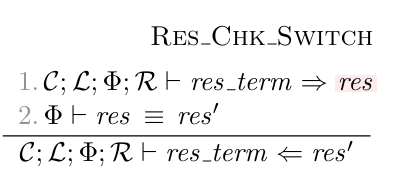
\includegraphics{figures/kernel-res-term-switch}
    \caption{Switching from checking to synthesising types for resource
        terms.}\label{fig:typing-res-term-switch}
\end{marginfigure}

\section{Memory actions and pointer operations}

As with resource terms, memory actions require all the contexts (computational,
logical, constraint and resource). The judgement $\mathcal{C} ; \mathcal{L} ;
\Phi ; \mathcal{R} \vdash \mathrm{mem\_action} \Rightarrow
\outpol{\mathrm{ret}}$ means that given the contexts and a memory action,
it synthesises a return type.

The rule for \coreinline{create()} is a bit busy because of % chktex 36
constraints on allocations required by the C standard (in premise 2), which I
will ignore. For now, the main thing to note is that the return type speaks of
the pointer to the newly created allocation as a computational value $y_p$,
constraints on pointer $y_p$ as required by the C standard, a unconstrained
logical (ghost) value for the pointee of the new allocation $x$, and the
finally the two resources it creates. The first is ownership of an
uninitialised piece of memory, at address $y_p$, and the second is an
allocation token $\mathsf{Alloc()}$ which is related to the memory object model
in \nameref{sec:cn-vip}.

In contrast, the rules for loads, stores and kill are quite simple. Loads
consume ownership of an initialised piece of memory\sidenote{For further
flexibility, loads of structs and unions could can be partially or completely
uninitialised, as allowed by the C standard, see
note~\ref{sn:partial-init-read}.}, check if the address of the load and the
address of the resource are symbolically equal, and synthesise a return type
mentioning the loaded value and ownership of the loaded location. Stores are
similar, but with extra checks on the stored value, which is also mentioned in
the ownership that is synthesised in the return type. Lastly, the rule for
\coreinline{kill()} is the converse of the one for \coreinline{create()}, % chktex 36
in that it \emph{consumes} the ownership and allocation token for a location
and synthesises a return type with no resources.\sidenote{I need to add the
rule for dynamic allocations.}

\begin{figure*}[tp]
    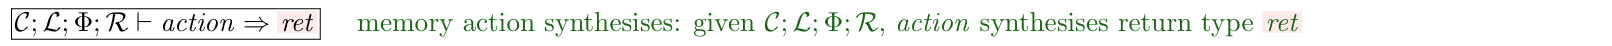
\includegraphics{figures/kernel-mem-action-typing-1}
    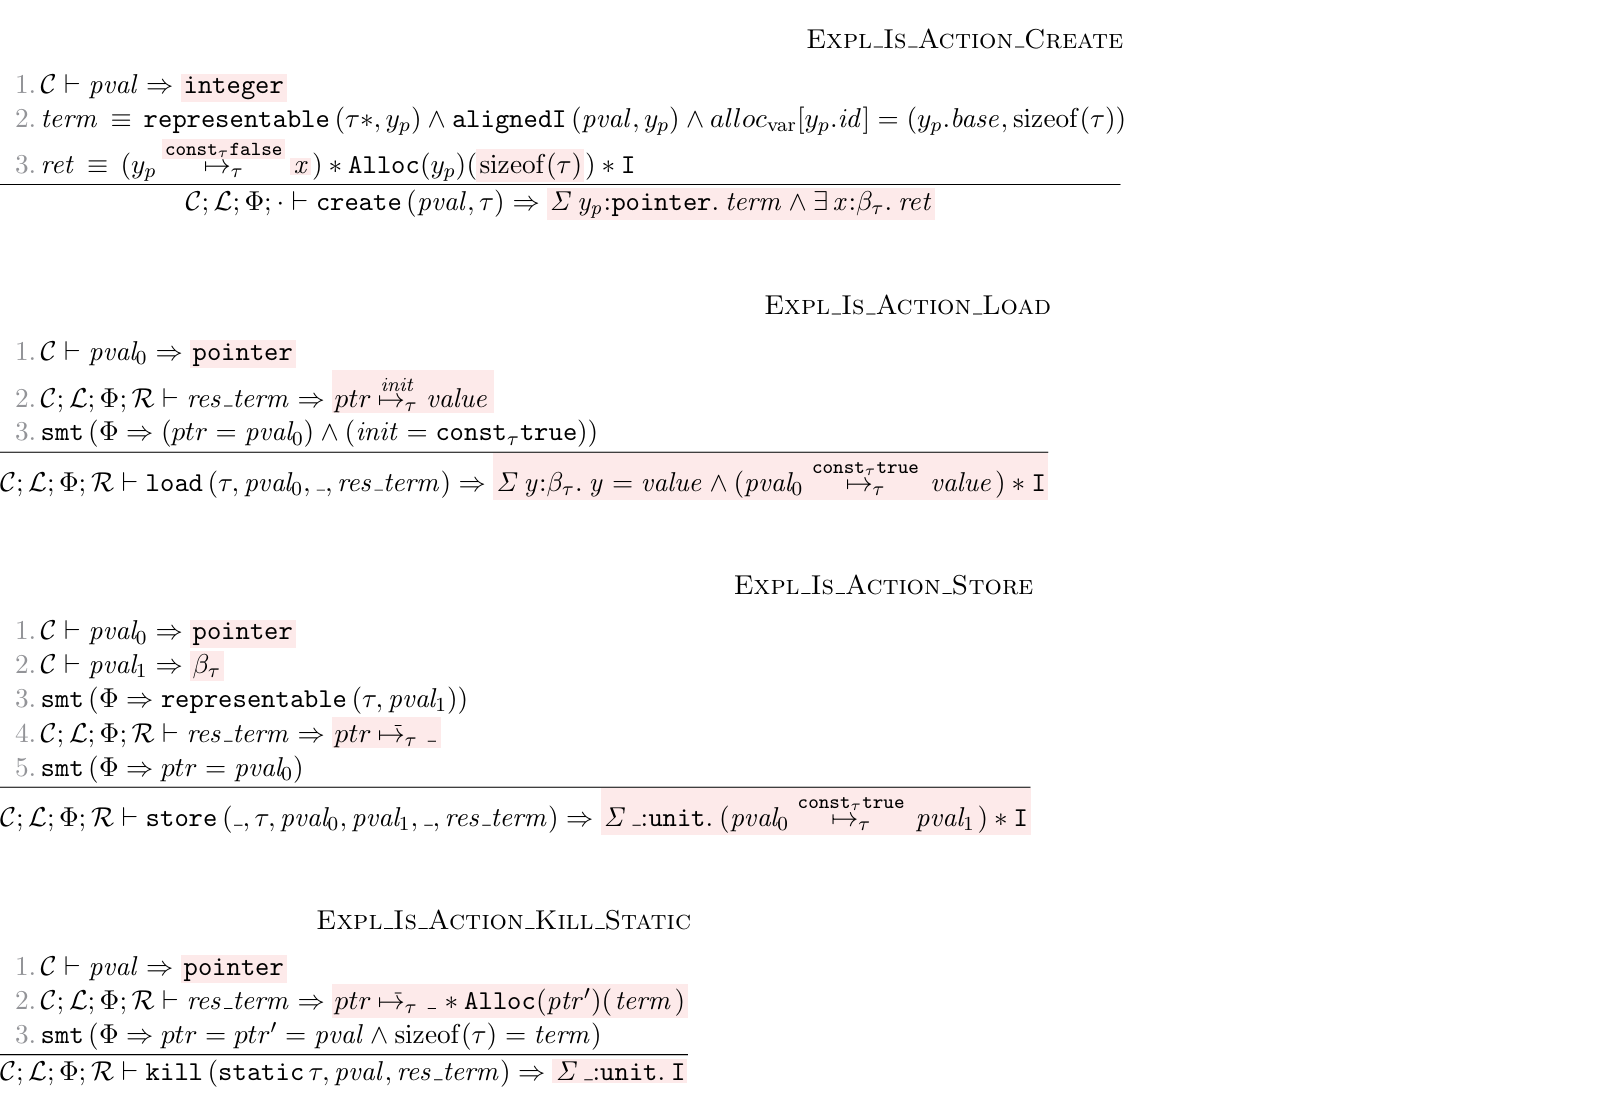
\includegraphics{figures/kernel-mem-action-typing-2}
    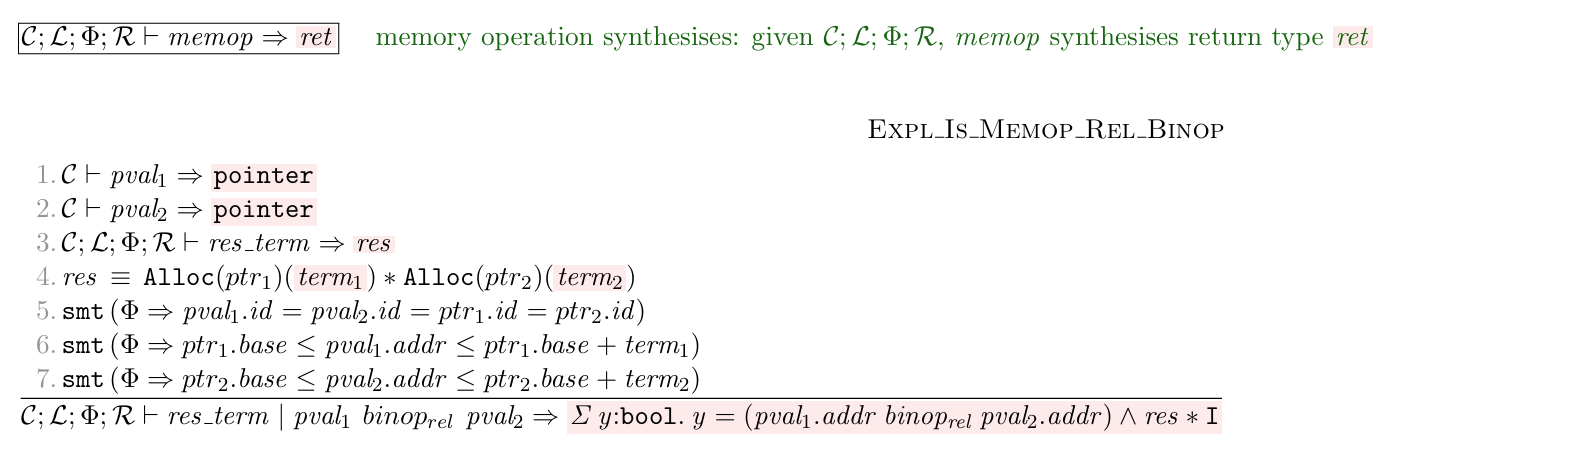
\includegraphics{figures/kernel-memop-typing}
    \caption{\kl{Kernel CN} typing rules for memory actions, and a select rule
        for typing a memory operation.}\label{fig:typing-mem-action}
\end{figure*}

Rules for typing memory operations, i.e.\ `effectful' pointer operations which
require not only for the pointer to be live, but satisfy certain allocation
bounds checks, also synthesise a return type. There are many of them, but they
share the same principles so it suffices to only explain one
(\cref{fig:typing-mem-action}).\sidenote{Update the rule to adjust the pointer
liveness check and notationally simplify the bounds checks into one line.}
Using a binary relational operator (not equality) is only valid if both
pointers are live, belong to the same allocation and have addresses which are
in that allocation's bounds. These constraints are all checked by the SMT
sovler, and the return type synthesises the result of that relational operator
applied to the addresses of those pointers, plus any resources consumed to
prove the pointer is live.

\section{Spine judgement}

There are two parts of the grammar which use spine, lists of values. The first
is its typical use in calls to pure Core functions, elaborated C functions, and
effectful Core procedures, as well as to the \coreinline{run()} % chktex 36
operator. Second is the less typical one, in \emph{top-level return values},
usually marked with \coreinline{done()}. So far, I have been showing % chktex 36
how expressions have return types, and so this is how to type the values to
which those expressions step.

Either way, the process for checking them is the same, and so the simplicity
gained by desugaring the \kl{CN} types into kernel types
(\cref{sec:desugaring}) pays off in the straightforward specification of these
rules (\cref{fig:typing-spine}).

\begin{figure*}[tp]
    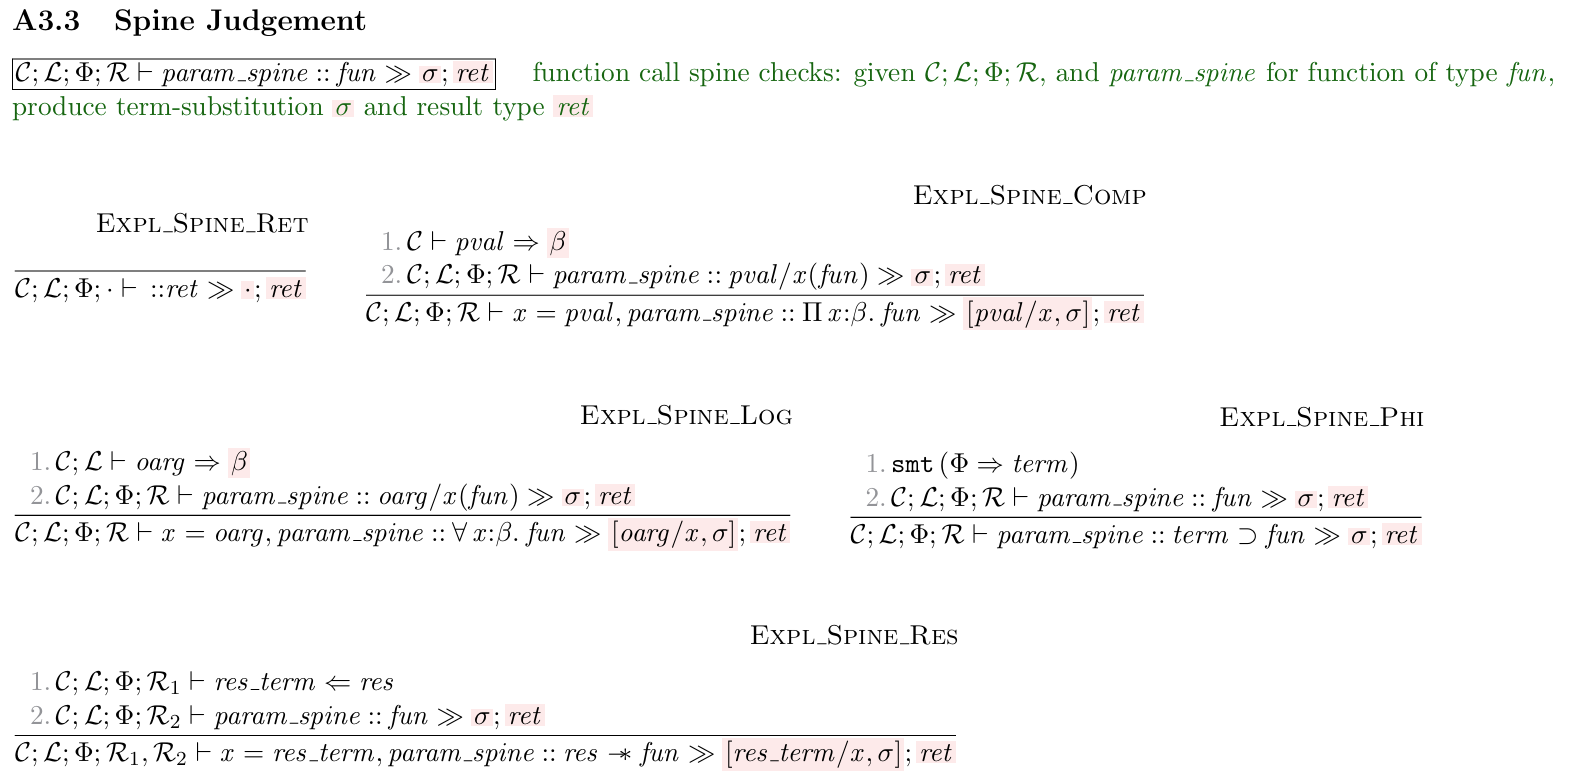
\includegraphics{figures/kernel-spine-typing}
    \caption{\kl{Kernel CN} typing rules for function
        spines.}\label{fig:typing-spine}
\end{figure*}

The judgement for typing spines is $\mathcal{C}; \mathcal{L}; \Phi ;
\mathcal{R} \vdash \mathit{param\_spine} \mathrel{{:}{:}} \mathit{fun} >\!\!>
\outpol{\sigma}; \outpol{ret}$, which means that given the contexts, a spine of
matched-up parameters and arguments and a function type, produce a substitution
$\sigma$ and a return type $\mathit{ret}$.

Function types are dependent over computational and logical (ghost) variables.
For notational convenience, I assume that the variables are the same as the
parameters in the spine. Typing these is done by substituting their
instantiation\sidenote{Remember that for \kl{kernel CN}, I assume all logical
(ghost) quantifiers are explicitly instantiated.} them into the type and typing
the rest of the spine. The substitution produced by this is extended with the
same.\sidenote{Building the substitution this way, rather than
`tail-recursively', made it easier to prove properties about it by induction
(\cref{sec:sub-ctxts}).}\label{sn:tail-rec-sub}. Constraints in types are
simply checked by the calling the SMT solver, and resources in types are
checked by splitting resource context, using one part to type the resource
term, and the other part to type the rest of the function type. Though these
types are not dependent over resources, the terms are, so this rule extends the
produced substitution with one for the resource too.

\section{Effectful values and expressions}

The spine typing is used in the rules for calling elaborated C function
\coreinline{ccall()}, and effectful Core procedures % chktex 36
\coreinline{pcall()}, in \cref{fig:typing-seq-expr-tval}. Both are % chktex 36
syntactically effectful sequenced expressions, typed with a judgement of the
form $\mathcal{C}; \mathcal{L}; \Phi; \mathcal{R} \vdash \mathit{seq\_expr}
\Rightarrow \outpol{ret}$, which says that given the contexts and an effectful
sequenced expression, synthesise a return type. Both lookup a function type for
the called function/procedure,\sidenote{\kl{CN} does not support
computed/indirect function calls, so I assume the callee has already been
resolved.} and simply produce the return type synthesised by the spine
judgement. This is also basically identical to how the top-level value
\coreinline{done<_>} is typed, with the main difference that (a) the judgement
$\mathcal{C}; \mathcal{L}; \Phi; \mathcal{R} \vdash \mathit{tval} \Leftarrow
\mathit{ret}$ is checking (b) the return type must be mapped to its dual
function type before using the spine judgement. Similar to the pure case, the
\coreinline{undef()} and \coreinline{error()} constructs % chktex 36 check
against any type if the constraint context is inconsistent.

\begin{figure*}[tp]
    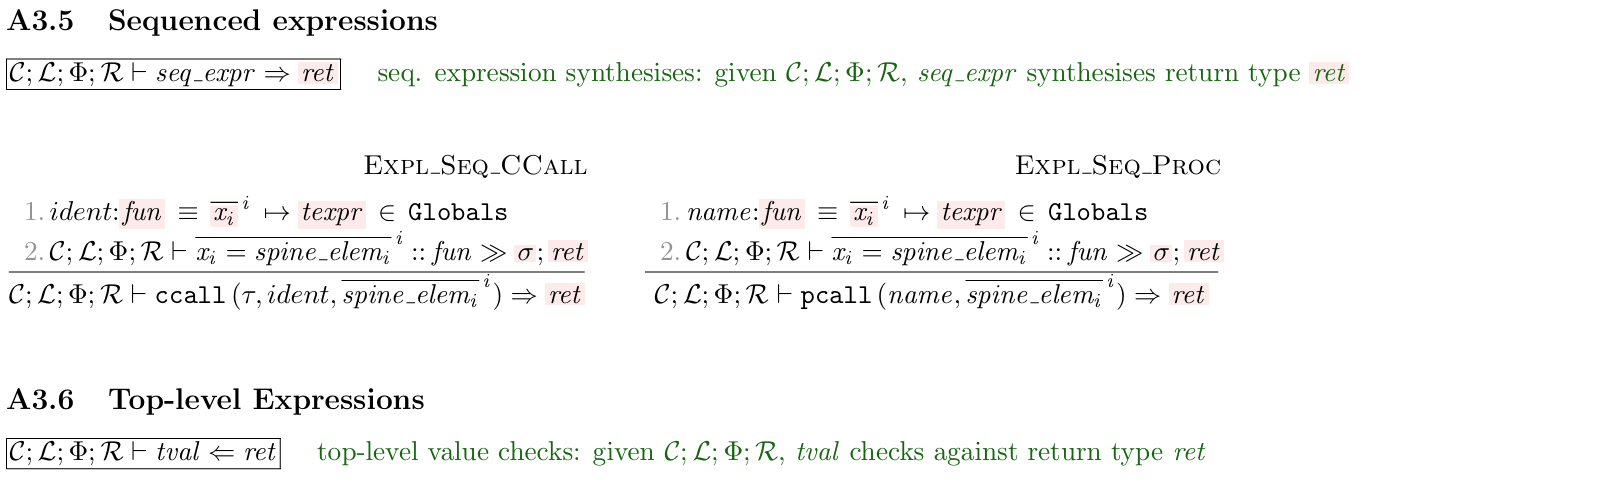
\includegraphics{figures/kernel-seq-expr-typing}
    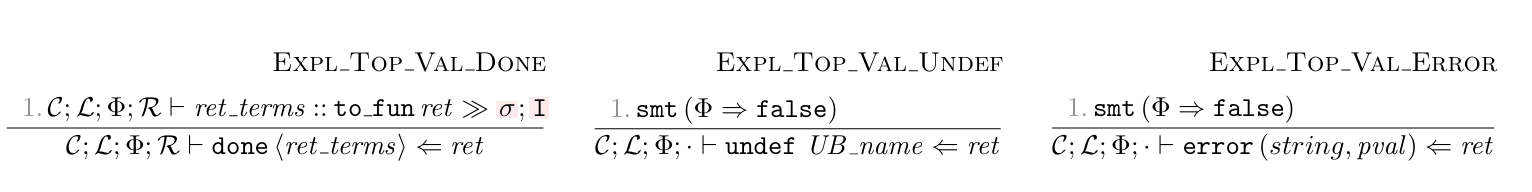
\includegraphics{figures/kernel-tval-typing}
    \caption{\kl{Kernel CN} typing rules for sequential expressions and top-level values.}\label{fig:typing-seq-expr-tval}
\end{figure*}

\section{Pattern matching}

Pattern matching is a surprisingly important crux of \kl{kernel CN}'s type
system because it \emph{is} the canal which directs a rich the grammar of
resource and return types into contexts. The judgement for this is
$\mathcal{C}; \mathcal{L}; \Phi \vdash \mathit{ret\_pat} {:} \mathit{ret}
\rightsquigarrow \outpol{\mathcal{C}'; \mathcal{L}'; \Phi'; \mathcal{R}'}$,
which says that given the contexts, a return pattern and a return type,
synthesise computational, logical, constraint and resource contexts.

Pattern matching for return types is complicated by the fact that they are
dependent on computational and logical (ghost) variables, and complicated
further by the fact that the computational values have their own patterns
(\cref{fig:typing-tpval-tpexpr}).

\begin{figure*}[tp]
    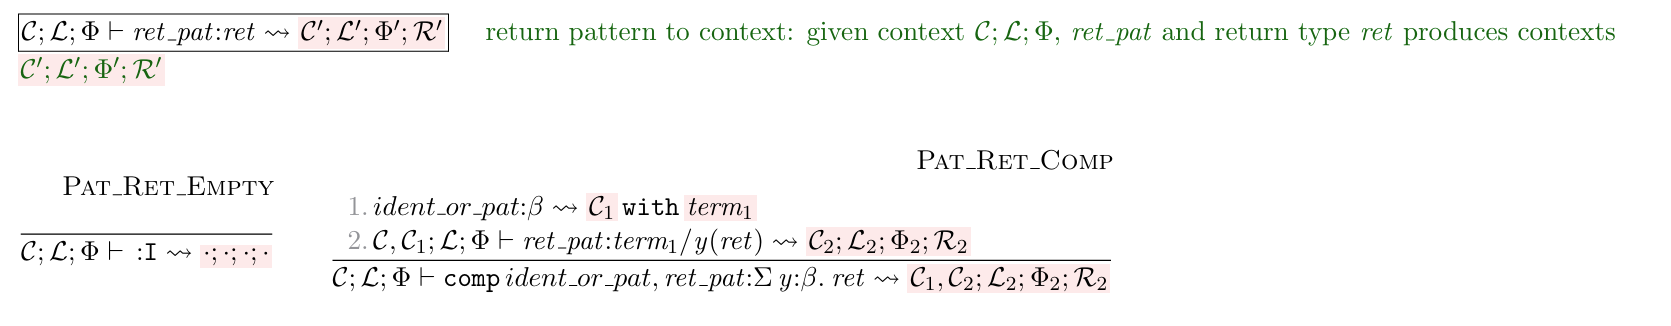
\includegraphics{figures/kernel-ret-pat-typing-1}
    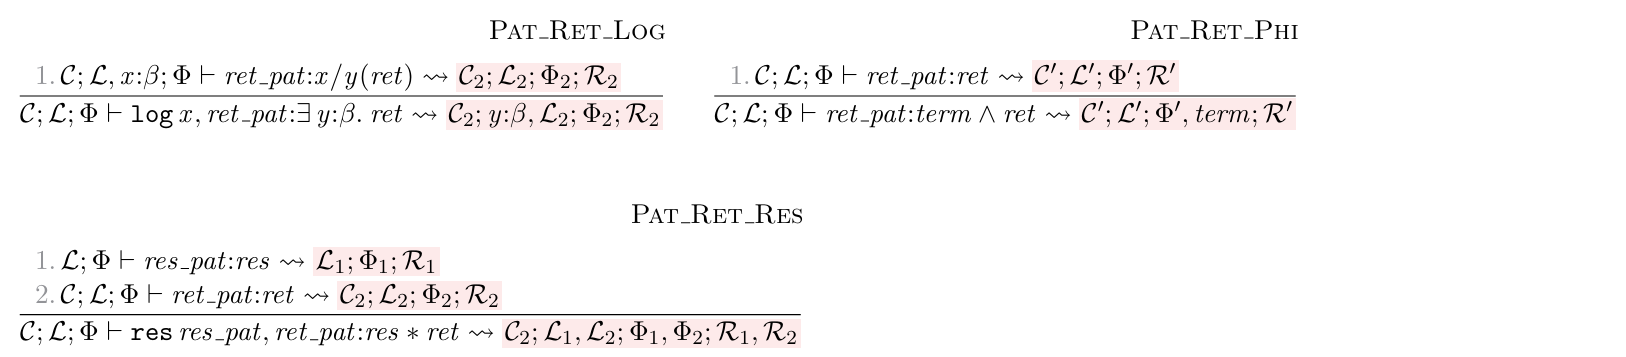
\includegraphics{figures/kernel-ret-pat-typing-2}
    \caption{\kl{Kernel CN} typing rules for pattern matching at return
        types.}\label{fig:typing-res-pat}
\end{figure*}

If both the head of the type and pattern are computational, the
\textsc{Pat\_Ret\_Comp} rule first uses the heads to synthesise a computational
context $\mathcal{C}_1$ and a represenative $\mathit{term}_1$ of the expected
shape. The former extends the input context, and the latter is substituted into
the the rest of the return type. After the remainder of the pattern is
converted into contexts, it is extended with $\mathcal{C}_1$.\sidenote{Similar
to what I mentioned in note~\ref{sn:tail-rec-sub} about substitution, I build
the contexts this way, rather than `tail-recursively', to make it easier to
prove properties about it by induction (\cref{sec:sub-ctxts}).}

If both the head of the return type and pattern are logical, then context is
extended with the pattern variable,\sidenote{\kl{CN} added support for
algebraic datatypes after I formalised \kl{kernel CN}
(\href{https://github.com/rems-project/cerberus/commit/0e5020732df2ec444ffa7a67abcc7c2c82904d24}{commit
0e50207}) and so and I did not formalise logical pattern matching; I would
formalise it identically to computational pattern matching.} and the same is
substituted into the rest of the return type. Similar to the computational
rule, the synthesised contexts is extended with the pattern variable.

Pattern matching for constraints simply adds the constraint to the contexts
synthesised by the rest of the return type for any pattern. And pattern
matching for resources similarly synthesises combines contexts from both the
resource type and pattern, and the rest of the return type and patterns.

This brings us on to how resource patterns synthesise contexts. The judgement
for this is $\mathcal{L}; \Phi \vdash \mathit{res\_pat}{:}\mathit{res}
\rightsquigarrow \outpol{\mathcal{L}'; \Phi'; \mathcal{R}'}$, which means that
given contexts,\sidenote{I abuse the notation slightly and omit the
computational context $\mathcal{C}$ because it remains the same in all the
rules.} a resource pattern and a type, synthesise logical, constraint and
resource contexts.

I am going to focus only on the rules for ordered-disjunctions and folds;
the rest are as expected.

\begin{figure*}[tp]
    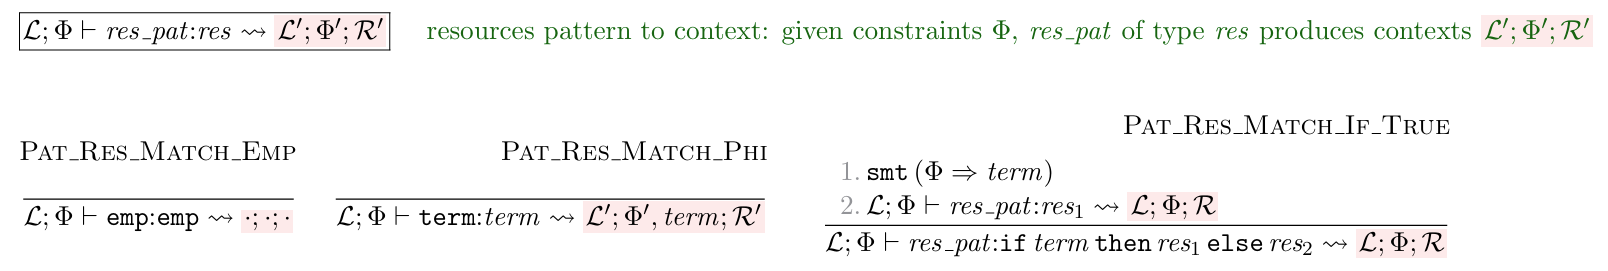
\includegraphics{figures/kernel-res-pat-typing-1}
    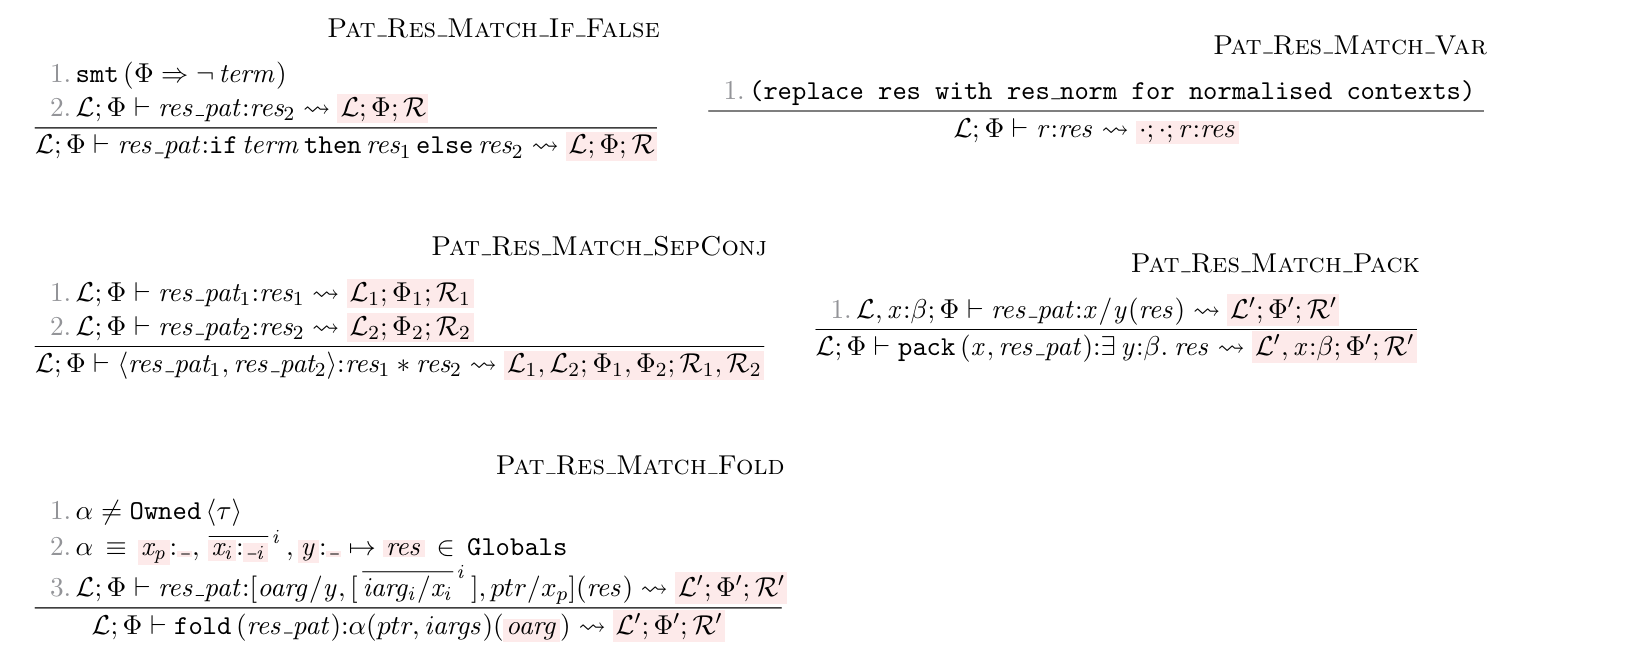
\includegraphics{figures/kernel-res-pat-typing-2}
    \caption{\kl{Kernel CN} typing rules for pattern matching at resource
        types.}\label{fig:typing-res-pat}
\end{figure*}

\section{Top-level effectful values and expressions}

\section{Elaboration}


\chapter{Kernel CN:\ Proof of soundness}%
\label{chap:kernel-soundness}

\section{Heaps and their types}\label{sec:heap-types}

\section{Substitution and contexts}\label{sec:sub-ctxts}

\chapter{Informing implementation discussions}\label{chap:inform-impl}

In the early stages, \kl{CN} was implemented by Christopher Pulte and Thomas
Sewell, based on sketches by Neel Krishnaswami. I started formalising
\kl{Kernel CN} much later, and benefited by the clarity of having an
implementations and implementers which and whom I could refer to in moments of
confusion.

However, this mode of development means that there were \emph{many} design
decisions made in a rather conservative context, because the programming was
always of a system which was being defined along the way, rather than a
well-understood pre-existing one. Extensions to syntax and inference were
always the minimum required for verifying the pKVM buddy allocator, lest
performance and inference suffer greatly, rather than ones based on a strong
formal and holistic consideration of the constructs and interactions at play.

As such, there are several restrictions in the implementation, which with the
benefit of hindsight and formalism, are completely unnecessary, but persist as
technical debt. This chapter list a few of these, and explains how the
formalisation brings much needed clarity to many questions around the
implementation.

\url{https://github.com/rems-project/cerberus/labels/language}
\url{https://github.com/rems-project/cerberus/labels/resource\%20reasoning}

\section{Supporting partially initialised reads of structs/unions}

This is not asked for, and actually seems to add a non-trivial amount of noise
and book-keeping to the formalisation. This suggests that the feature is not
worth implementing in CN unless a strong use-case comes up.

\section{Auto unfolding scheme for logical functions}
\url{https://github.com/rems-project/cerberus/issues/483}

\section{Higher-order resources}
\url{https://github.com/rems-project/cerberus/issues/483}

\section{Restrictions on branching}\label{sec:restriction-branching}
\url{https://github.com/rems-project/cerberus/issues/483}
\url{https://github.com/rems-project/cerberus/issues/266}

\section{Removing the pointer first restriction on predicates}\label{sec:rm-ptr-first}
\url{https://github.com/rems-project/cerberus/issues/303}

\section{Unifying the syntax of functions, predicates and specifications}
\url{https://github.com/rems-project/cerberus/issues/304}


\chapter{An alternative presentation}\label{chap:kernel-alternative}

Perhaps a short chapter about MiniCN\@? This could demonstrate the strong
advantages of defining a type system over a first-order functional language,
rather than trying to do so directly over something C-like.

It would also give some space to the interesting but yet-to-be-baked ideas
from the Fuliminate paper.


